\subsection{Thực nghiệm mở rộng: Tái cấu trúc không gian nhãn}
\label{subsec:extended_rebalanced_experiment}

Để kiểm tra liệu một phần lỗi của baseline có đến từ sự phân mảnh và mất cân bằng của không gian nhãn gốc hay không, một thực nghiệm mở rộng được thực hiện trên phiên bản nhãn đã tái cấu trúc. Trong FoodSeg103, một số lớp có rất ít mẫu, trong khi nhiều nhóm nguyên liệu lại gần nhau về ngữ nghĩa và texture sau chế biến, khiến mô hình nhẹ khó phân biệt các ranh giới thị giác mờ. Vì vậy, các lớp có quan hệ ngữ nghĩa gần và độ tương đồng texture cao được gộp lại nhằm giảm nhiễu nhãn. Thực nghiệm này không thay thế đánh giá trên bài toán gốc, mà đóng vai trò phân tích bổ sung để làm rõ ảnh hưởng của cấu trúc nhãn đến lỗi của BiSeNet.

Sử dụng đặc trưng texture dựa trên ma trận đồng xuất hiện mức xám (GLCM) để gôm lớp. Với mỗi lớp con $k$, các vùng ảnh thuộc lớp đó được dùng để tính vector texture trung bình $\mathbf{f}_k$, gồm các đặc trưng như contrast, homogeneity, energy và correlation. Độ tương đồng giữa hai lớp $i$ và $j$ được đo bằng cosine similarity $ \mathrm{Sim}(i,j) =
\frac{\mathbf{f}_i \cdot \mathbf{f}_j}
{\|\mathbf{f}_i\| \|\mathbf{f}_j\|}.$

Hai lớp chỉ được xem xét gộp khi chúng đồng thời thỏa mãn hai điều kiện: gần nhau về mặt ngữ nghĩa và có mức tương đồng texture đủ cao. Trong thực nghiệm này, ngưỡng tương đồng được đặt là $\mathrm{Sim}(i,j) \geq 0.85$. Cách làm này giúp hạn chế việc gộp các lớp không liên quan, đồng thời bảo toàn ý nghĩa thị giác của nhãn sau khi gộp.

\begin{figure}[H]
    \centering
    \begin{subfigure}{0.48\linewidth}
        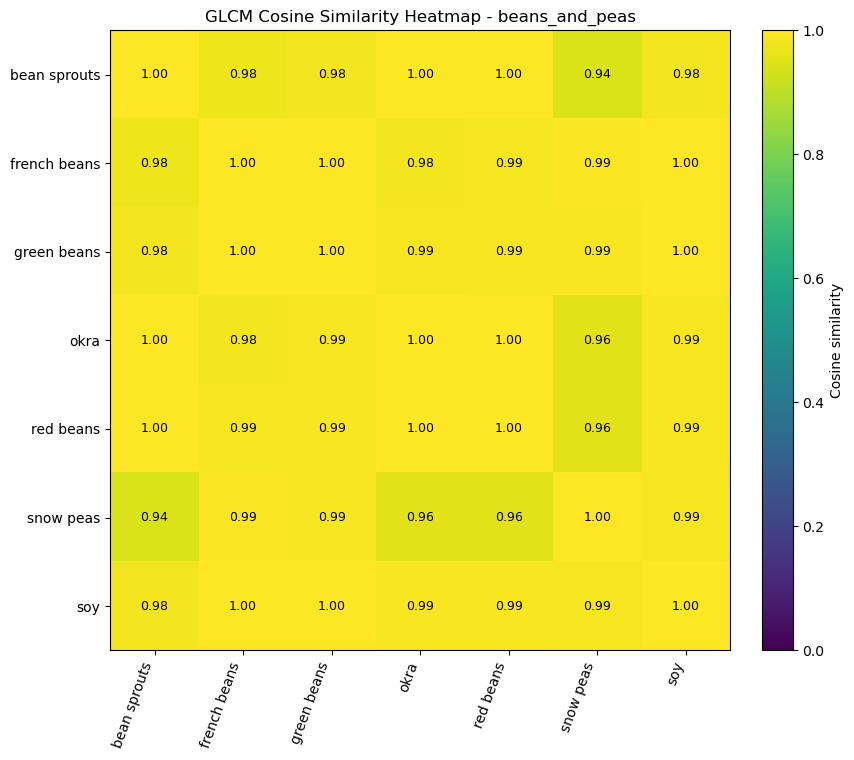
\includegraphics[width=\linewidth]{img/analyze/bean_.png}
        \caption{Beans and peas.}
    \end{subfigure}
    \hfill
    \begin{subfigure}{0.48\linewidth}
        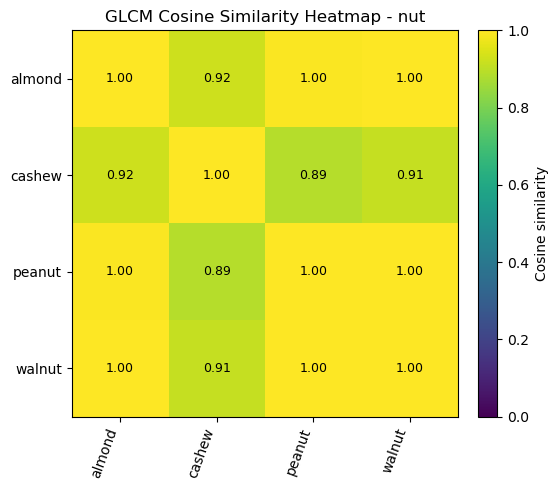
\includegraphics[width=\linewidth]{img/analyze/nut.png}
        \caption{Nuts.}
    \end{subfigure}
    \caption{Ví dụ ma trận cosine similarity dựa trên đặc trưng GLCM giữa các lớp con trong thực nghiệm tái cấu trúc nhãn.}
    \label{fig:glcm_similarity}
\end{figure}

Bảng~\ref{tab:merge_groups} trình bày một số nhóm lớp được gộp trong thực nghiệm mở rộng. Ví dụ, các loại nấm khác nhau được ánh xạ về \texttt{mushroom}; các lớp như \texttt{green beans}, \texttt{french beans}, \texttt{snow peas} và \texttt{bean sprouts} được gộp thành \texttt{beans\_and\_peas}. Đây là các nhóm có quan hệ ngữ nghĩa gần và có khả năng gây nhiễu nếu mô hình phải phân biệt ở mức quá chi tiết trong điều kiện dữ liệu hạn chế.

\begin{table}[H]
\centering
\caption{Một số nhóm lớp được gộp trong thực nghiệm mở rộng}
\label{tab:merge_groups}
\begin{tabular}{p{0.56\linewidth}p{0.30\linewidth}}
\toprule
\textbf{Nhóm lớp gốc} & \textbf{Lớp sau khi gộp} \\
\midrule
king oyster mushroom, oyster mushroom, enoki mushroom, white button mushroom, shiitake 
& \texttt{mushroom} \\
\midrule
green beans, french beans, snow peas, bean sprouts, soy, red beans, okra 
& \texttt{beans\_and\_peas} \\
\midrule
peanut, almond, cashew, walnut 
& \texttt{nut} \\
\midrule
cake, biscuit, pudding, egg tart, candy, chocolate, popcorn 
& \texttt{desserts} \\
\midrule
lemon, orange 
& \texttt{citrus} \\
\midrule
spring onion, onion, garlic, ginger 
& \texttt{alliums\_and\_garlic} \\
\midrule
cabbage, rape, lettuce 
& \texttt{leafy\_greens} \\
\midrule
kelp, seaweed
& \texttt{seaweed} \\
\bottomrule
\end{tabular}
\end{table}

Sau khi tái cấu trúc, không gian nhãn giảm từ 103 lớp xuống còn 75 lớp. Bộ dữ liệu tạo ra trong thực nghiệm mở rộng được gọi là \texttt{FoodSeg103\_rebalanced}. Về số lượng ảnh, tập train giảm từ 3982 xuống 3981 ảnh do một ảnh lỗi tệp, trong khi tập test giữ nguyên 2135 ảnh. Không có ảnh nào bị loại do mask rỗng sau ánh xạ nhãn.

\begin{table}[H]
    \centering
    \caption{Thống kê dữ liệu trong thực nghiệm mở rộng}
    \label{tab:data_before_after}
    \begin{tabular}{lrr}
        \toprule
        \textbf{Chỉ số} & \textbf{FoodSeg103 gốc} & \textbf{FoodSeg103\_rebalanced} \\
        \midrule
        Số lớp mục tiêu & 103 & 75 \\
        Số ảnh train & 3982 & 3981 \\
        Số ảnh test & 2135 & 2135 \\
        \bottomrule
    \end{tabular}
\end{table}

\begin{figure}[H]
    \centering
    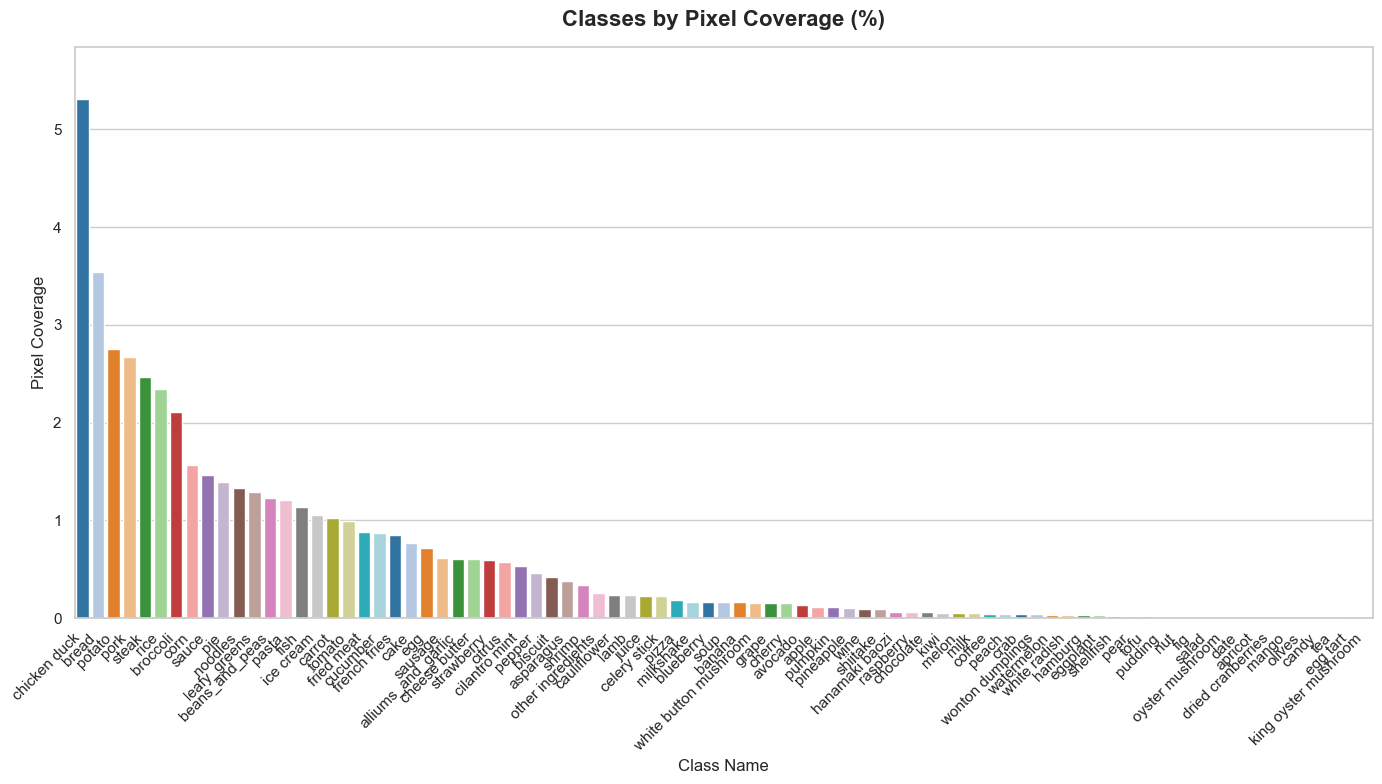
\includegraphics[width=\linewidth]{img/analyze/graph_after.png}
    \caption{Mức bao phủ pixel theo lớp sau khi tái cấu trúc không gian nhãn trong thực nghiệm mở rộng.}
    \label{fig:pixel_coverage_after}
\end{figure}

Kết quả của thực nghiệm này được sử dụng để hỗ trợ phân tích lỗi của baseline. Nếu việc giảm phân mảnh nhãn giúp mô hình ổn định hơn, điều đó cho thấy một phần khó khăn của FoodSeg103 đến từ không gian nhãn quá chi tiết và không cân bằng. Tuy nhiên, long-tail vẫn chưa biến mất hoàn toàn sau khi gộp lớp, do đó đây không phải là giải pháp cuối cùng. Thay vào đó, thực nghiệm này củng cố nhu cầu thiết kế mô hình có khả năng xử lý đồng thời hai vấn đề: phân biệt texture cục bộ giữa các nguyên liệu gần nhau và điều chỉnh dự đoán theo quan hệ đồng xuất hiện giữa các lớp.